\subsection{Integration archetypes}

Equivalences between data types and the automated process enables to create integration archetypes based on classes CLUSTER and ELEMENT. These integration ar\-chetypes serve the main purpose of being the entry point of the semantic conversion process for data import to open\-EHR systems. Figure \ref{fig:comparison} shows an extract of a patient integration archetype from side to side, created using the automated process and the patient FHIR resource from which it was created.

\begin{figure*}
  \centering
  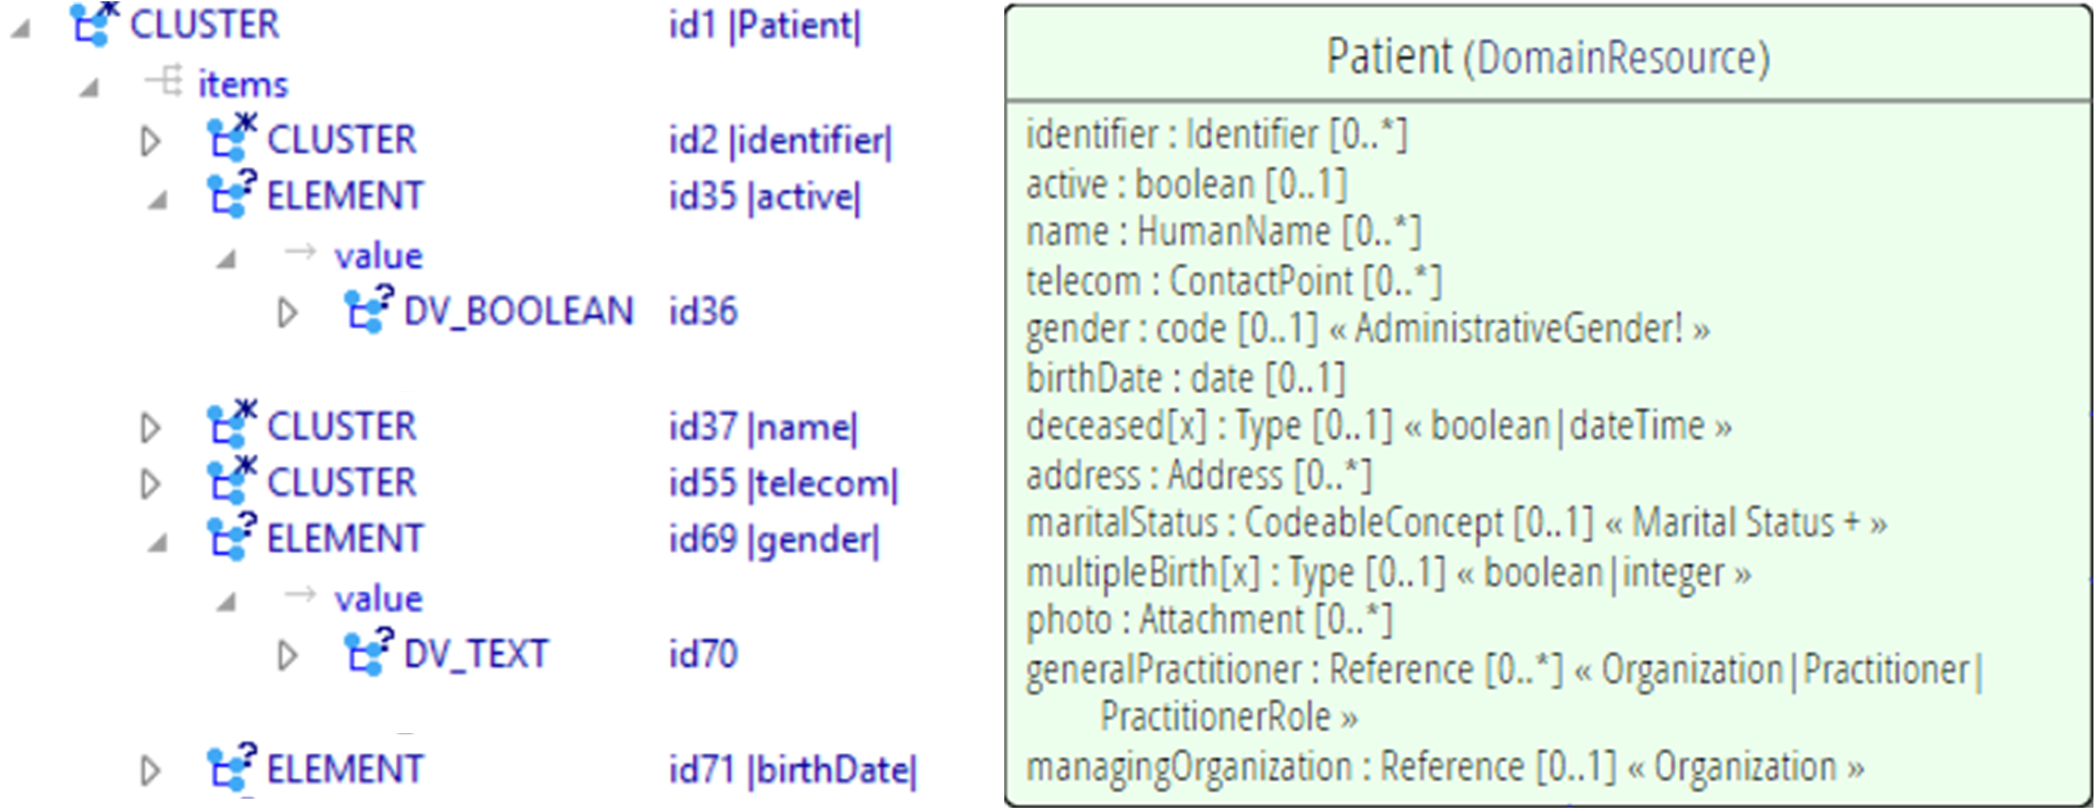
\includegraphics[scale=0.8]{./images/comparison_patient}
  \caption{Comparison of a patient integration archetype and a patient FHIR resource.}
  \label{fig:comparison}
\end{figure*}
